\chapter{Results}

\section{Deuteron photodisintegraion}
    % \label{sec:deut_bound}

    \begin{figure}[h]
        \begin{center}
        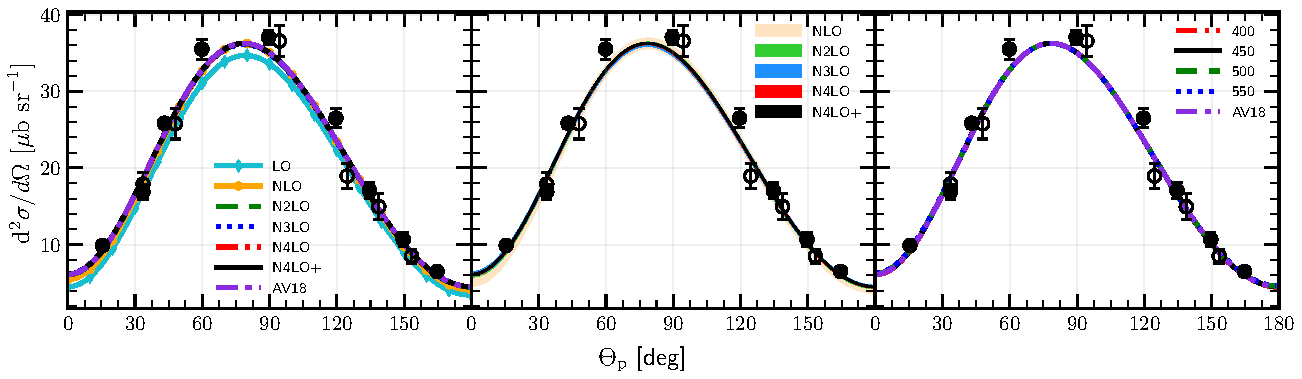
\includegraphics[width=0.95\textwidth]{Figures_python/CROSS2_30mev.pdf}
        \end{center}
        \caption{Differential cross section as a dependence on the outgoing proton angle in the center of mass frame 
        for the photon's energy 30 MeV. Left figure presents results obtained using potential
        with different chiral orders (from LO to N$^4$LO+) with cutoff parameter $\Lambda=450$~MeV
        whereas right figure presents a cutoff dependency and chiral potential N$^4$LO+ was used in all cases.
        For the sake of comparison, predictions obtained with AV18 potential are on both figures as well.}
        \label{CROSS_30}
    \end{figure}
        

    \begin{figure}[h]
        \begin{center}
        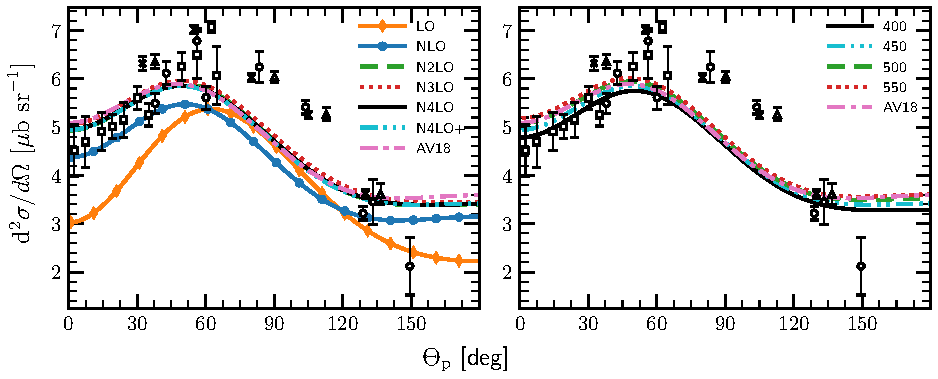
\includegraphics[width=0.95\textwidth]{Figures_python/CROSS2_100mev.pdf}
        \end{center}
        \caption{The same as on the Fig.~\ref{CROSS_30} but for the photon's energy E$_\gamma$=100~MeV}
        \label{CROSS_100}
    \end{figure}

    \begin{figure}[h]
        \begin{center}
        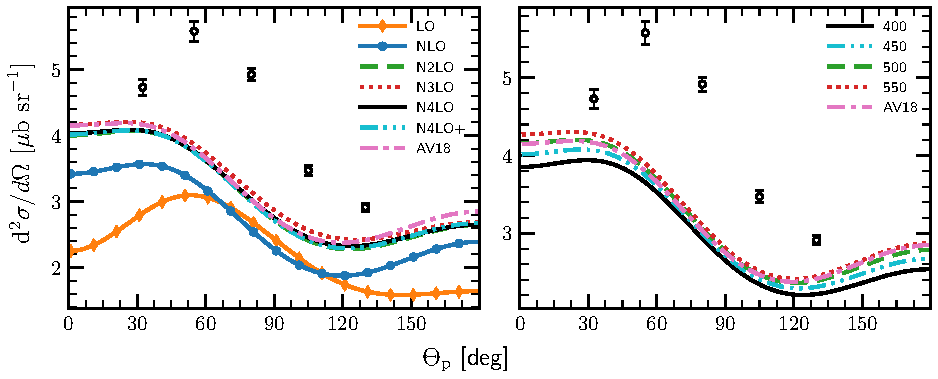
\includegraphics[width=0.95\textwidth]{Figures_python/CROSS2_140mev.pdf}
        \end{center}
        \caption{The same as on the Fig.~\ref{CROSS_30} but for the photon's energy E$_\gamma$=140~MeV}
        \label{CROSS_140}
    \end{figure}
        


    \begin{figure}[h]
        \begin{center}
        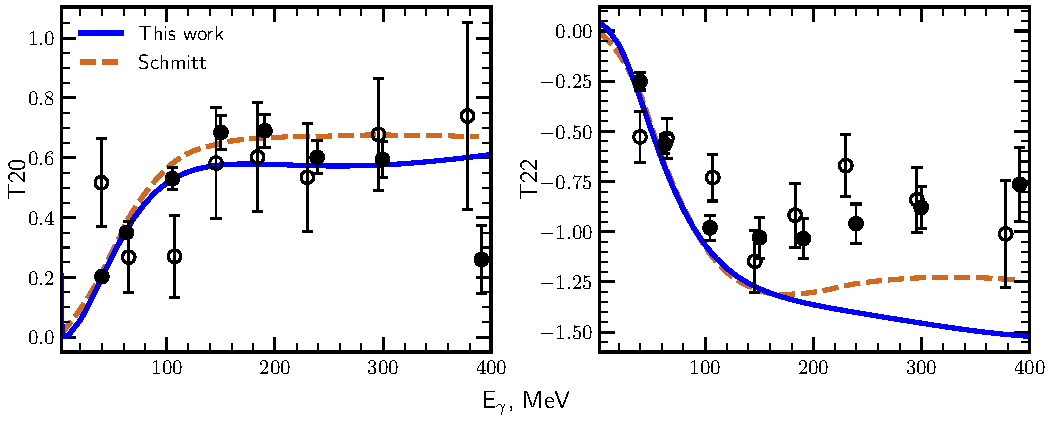
\includegraphics[width=0.95\textwidth]{Figures_python/T20_T22_vs_en.pdf}
        \end{center}
        \caption{Tensor analyzing powers T$_{20}$ and T$_{22}$ as a functions of the photon energy E$_\gamma$
        with fixed outgoing proton angle $\theta_p = 88^{\circ}$ (in the center of mass frame).
        My predictions (solid line) are obtained with SMS potential at chiral order N$^4$LO+
        and with cutoff parameter $\Lambda$~=~450~MeV.
        Dashed line presents calculations  from \cite{Schmitt1989}.
        Experimental data is taken from \cite{rachek2007} (filled circles)
        and \cite{mishev1993} (empty squares).}
        \label{T20_vs_en}
    \end{figure}


    \begin{figure}[h]
        \begin{center}
        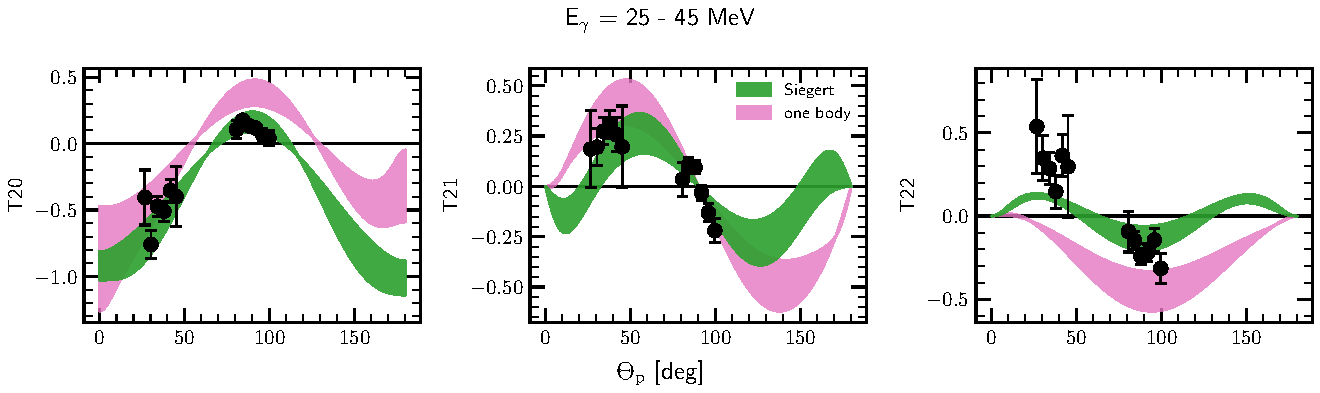
\includegraphics[width=0.95\textwidth]{Figures_python/Tensor_analyzing_power_angular_E25-45.pdf}
        \end{center}
        \caption{Tensor analyzing powers T$_{20}$, T$_{21}$ and T$_{22}$ as a functions of the
        outgoing proton angle $\theta_p$ (in the center of mass frame).
        Filled bands show maximal spread of my predictions obtained with a 
        SMS potential at N$^4$LO+ chiral order and with $\Lambda$~=~450~MeV
        for the energy span from 25 to 45 MeV. Filled circles is experimental data
        from \cite{rachek2007} for the analogous energy span.}
        % My predictions (solid line) are obtained with SMS potential at chiral order N$^4$LO+
        % and with cutoff parameter $\Lambda$~=~450~MeV.
        % Dashed line presents calculations  from \cite{Schmitt1989}.
        % Experimental data is taken from \cite{rachek2007} (filled circles)
        % and \cite{mishev1993} (empty squares).}
        \label{tensor_angular_25-45}
    \end{figure}

    \begin{figure}[h]
        \begin{center}
        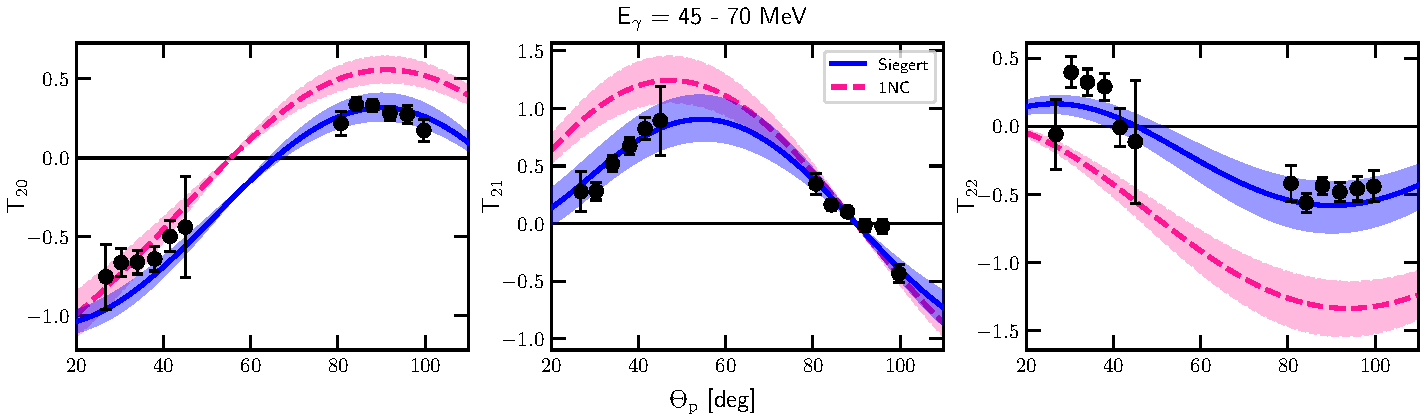
\includegraphics[width=0.95\textwidth]{Figures_python/Tensor_analyzing_power_angular_E45-70.pdf}
        \end{center}
        \caption{The same as on \ref*{tensor_angular_25-45} but for energy bin 45~-~70~MeV}
        \label{tensor_angular_45-70}
    \end{figure}

    \begin{figure}[h]
        \begin{center}
        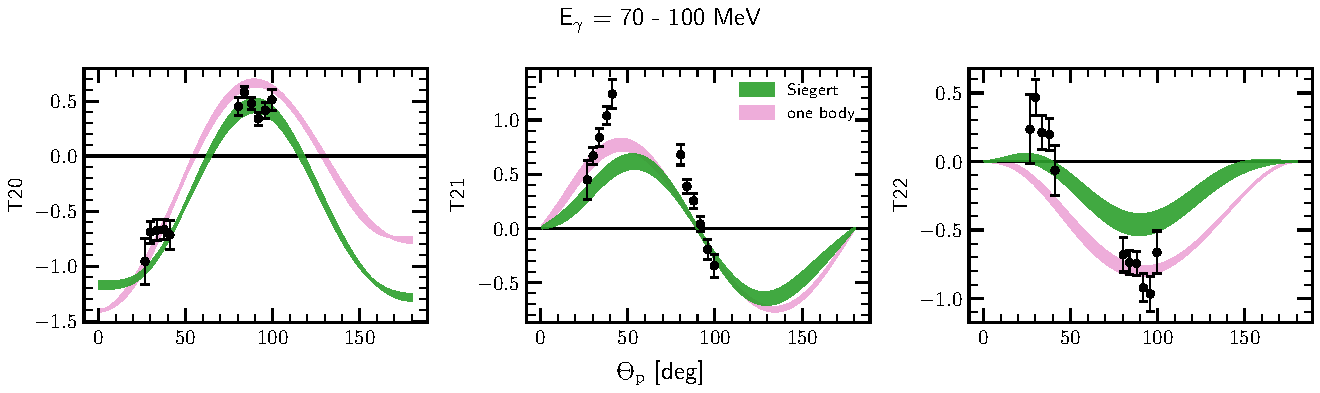
\includegraphics[width=0.95\textwidth]{Figures_python/Tensor_analyzing_power_angular_E70-100.pdf}
        \end{center}
        \caption{The same as on \ref*{tensor_angular_25-45} but for energy bin 70~-~100~MeV}
        \label{tensor_angular_70-100}
    \end{figure}

    \begin{figure}[h]
        \begin{center}
        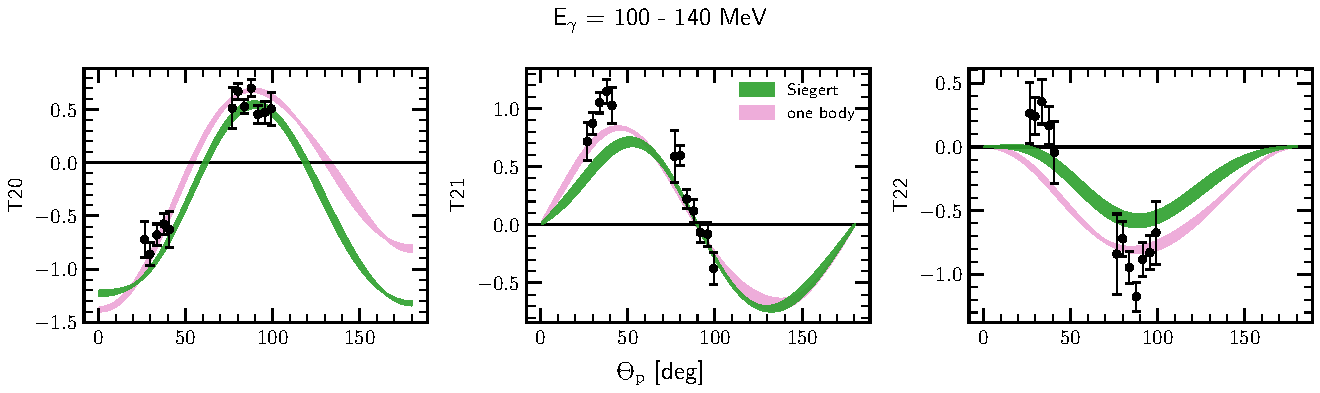
\includegraphics[width=0.95\textwidth]{Figures_python/Tensor_analyzing_power_angular_E100-140.pdf}
        \end{center}
        \caption{The same as on \ref*{tensor_angular_25-45} but for energy bin 100~-~140~MeV}
        \label{tensor_angular_70-100}
    \end{figure}
        